\section{\trNaturalEquivalence{}的\trPointwise{}判别法}
\label{sec:pointwise-criterion}

本节的目标是证明：设 $f, g\colon \C \to \D$ 是∞-\trCategories{}之间的%
\trFunctor{}，而 $\tau$ 是其间的\trNaturalTransformation{}；如果 $\tau$ \trPointwise{}地
是\trEquivalence{}，那么把它视作\trFunctor{}∞-\trCategory{}%
$\mathrm{Fun}(\C, \D)$ 中的\trMorphism{}时，它本身就是\trEquivalence{}。与%
\trOrdinaryCategory{}的情形不同——在那里，\trPointwise{}取唯一的逆，容易看出这些逆能拼装成一个逆%
\trNaturalTransformation{}——在∞-\trCategories{}的情形下，这一点毫不显然。
因此，我们需要证明下述定理。

\begin{theorem}\label{thm:bijective-on-vertices}
设 $L \to K$ 是\trSimplicialSets{}之间的一个映射，它诱导一个双射
$L_0 \to K_0$。那么，对每个∞-\trCategory{} $\C$，诱导\trFunctor{}%
\[
\mathrm{Fun}(K, \C) \longrightarrow \mathrm{Fun}(L, \C)
\]
是\trConservative。
\end{theorem}

\begin{corollary}\label{cor:pointwise-equivalences}
典范\trFunctor{}%
\[
\mathrm{Fun}(K, \C) \longrightarrow \prod_{x \in K_0} \C
\]
是\trConservative。换言之，设 $f\colon \Delta^1 \to \mathrm{Fun}(K, \C)$ 是两个%
\trFunctor{} $F, G\colon K \to \C$ 之间的\trNaturalTransformation{}。如果对所有
$x \in K_0$，诱导的\trMorphism{} $\Delta^1 \to \C$ 都是\trEquivalence{}，那么
$f$ 是一个\trEquivalence{}。\footnote{译注：原书印作「对所有 $x \in K$」，但依
上下文（右边的乘积取遍 $x \in K_0$，且 $\Delta^1 \to \C$ 指 $F$ 与 $G$ 在顶点
$x$ 处的取值之间的\trMorphism{}），应为 $x \in K_0$，兹径改。——译者注}
\end{corollary}

为了证明\cref{thm:bijective-on-vertices}，我们观察到：只需处理%
\cref{cor:pointwise-equivalences} 的情形即可，此时 $L \to K$ 取为映射
$K_0 \to K$，其中 $K_0 = \mathrm{sk}_0(K)$ 是由 $K$ 的零\trSimplex{}构成的
离散\trSimplicialSet{}。考虑图表
\begin{center}
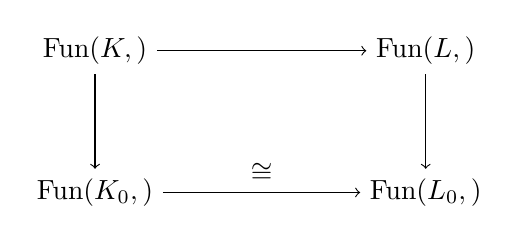
\begin{tikzpicture}
  \node (fk) at (0,0) {$\mathrm{Fun}(K, \C)$};
  \node (fl) at (4.2,0) {$\mathrm{Fun}(L, \C)$};
  \node (fk0) at (0,-1.8) {$\mathrm{Fun}(K_0, \C)$};
  \node (fl0) at (4.2,-1.8) {$\mathrm{Fun}(L_0, \C)$};
  \draw[->] (fk) -- (fl);
  \draw[->] (fk) -- (fk0);
  \draw[->] (fl) -- (fl0);
  \draw[->] (fk0) -- node[above] {$\cong$} (fl0);
\end{tikzpicture}
\end{center}
便可立刻看出这一点：其中下面的水平\trFunctor{}是一个同构，而竖直的诸%
\trFunctor{}由假设是\trConservative。由此得出，上面的水平\trFunctor{}也是%
\trConservative。

在这一情形中，我们考虑 $K$ 上的\trSkeleton{}滤过，得到一个由\trSimplicialSets{}构成的塔
\[
\dotsb \longrightarrow \mathrm{Fun}(\mathrm{sk}_n(K), \C)
\longrightarrow \mathrm{Fun}(\mathrm{sk}_{n-1}(K), \C)
\longrightarrow \dotsb \longrightarrow
\mathrm{Fun}(\mathrm{sk}_0(K), \C),
\]
其\trInverseLimit{}为 $\mathrm{Fun}(K, \C)$。注意，上述塔中出现的所有映射由
\cref{thm:angle-fi-fibration} 都是\trInnerFibration{}。

我们首先证明：如果诸\trFunctor{}%
$\mathrm{Fun}(\mathrm{sk}_n(K), \C) \to \mathrm{Fun}(\mathrm{sk}_{n-1}(K), \C)$
中的每一个都是\trConservative，那么\trFunctor{}%
$\mathrm{Fun}(K, \C) \to \mathrm{Fun}(\mathrm{sk}_0(K), \C)$ 是\trConservative。为
此，我们希望使用\cref{cor:conservative-special-horn} 来证明\trFunctor{}%
$\mathrm{Fun}(K, \C) \to \mathrm{Fun}(K_0, \C)$ 是\trConservative。于是我们考虑一个%
\trLiftingProblem{}%
\begin{center}
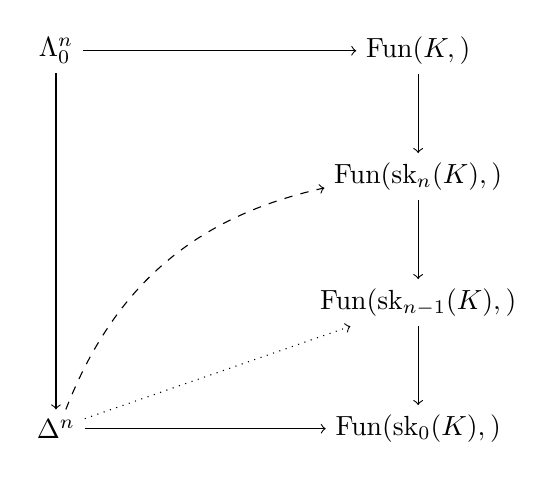
\begin{tikzpicture}
  \node (l) at (0,0) {$\Lambda^n_0$};
  \node (r1) at (4.6,0) {$\mathrm{Fun}(K, \C)$};
  \node (r2) at (4.6,-1.6) {$\mathrm{Fun}(\mathrm{sk}_n(K), \C)$};
  \node (r3) at (4.6,-3.2) {$\mathrm{Fun}(\mathrm{sk}_{n-1}(K), \C)$};
  \node (r4) at (4.6,-4.8) {$\mathrm{Fun}(\mathrm{sk}_0(K), \C)$};
  \node (d) at (0,-4.8) {$\Delta^n$};
  \draw[->] (l) -- (r1);
  \draw[->] (r1) -- (r2);
  \draw[->] (r2) -- (r3);
  \draw[->] (r3) -- (r4);
  \draw[->] (l) -- (d);
  \draw[->] (d) -- (r4);
  \draw[->, dashed] (d) to[bend left=28] (r2);
  \draw[->, dotted] (d) -- (r3);
\end{tikzpicture}
\end{center}
其中特殊边 $\Delta^{[0,1]} \subseteq \Lambda^n_0$ 被送到
$\mathrm{Fun}(\mathrm{sk}_0(K), \C)$ 中的一个\trEquivalence{}。我们希望归纳地
证明：给定点箭头，便能构造出虚箭头，使得所有图表都交换。这可以由
\cref{cor:conservative-special-horn} 以及「由
$\mathrm{sk}_{n-1}(K) \to \mathrm{sk}_n(K)$ 诱导的那些映射是\trConservative」这一假设
来完成。

还须证明：对 $n \ge 1$，诸\trFunctor{}%
$\mathrm{Fun}(\mathrm{sk}_n(K), \C) \to \mathrm{Fun}(\mathrm{sk}_{n-1}(K), \C)$
事实上是\trConservative。存在\trPullback{}图表
\begin{center}
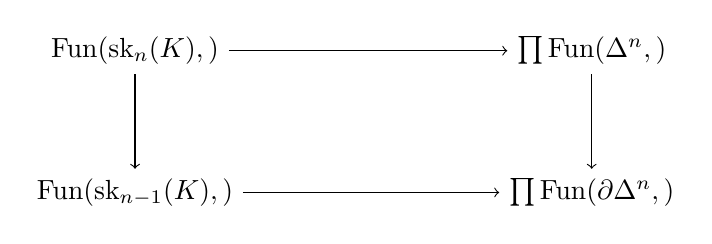
\begin{tikzpicture}
  \node (a) at (0,0) {$\mathrm{Fun}(\mathrm{sk}_n(K), \C)$};
  \node (b) at (5.8,0) {$\prod \mathrm{Fun}(\Delta^n, \C)$};
  \node (c) at (0,-1.8) {$\mathrm{Fun}(\mathrm{sk}_{n-1}(K), \C)$};
  \node (e) at (5.8,-1.8) {$\prod \mathrm{Fun}(\partial \Delta^n, \C)$};
  \draw[->] (a) -- (b);
  \draw[->] (a) -- (c);
  \draw[->] (b) -- (e);
  \draw[->] (c) -- (e);
\end{tikzpicture}
\end{center}
由于\trConservative{}\trFunctor{}的乘积是\trConservative，所有竖直映射都是%
\trInnerFibration{}，而\trConservative{}\trInnerFibration{}的\trPullback{}是%
\trConservative，所以只需证明：对每个
$n \ge 1$，\trFunctor{}%
\[
\mathrm{Fun}(\Delta^n, \C) \longrightarrow \mathrm{Fun}(\partial \Delta^n, \C)
\]
是\trConservative。首先处理 $n \ge 2$ 的情形。此时，包含 $I^n \to \Delta^n$ 经过
$\partial \Delta^n$ 分解，故我们可以考虑复合
\[
\mathrm{Fun}(\Delta^n, \C) \longrightarrow \mathrm{Fun}(\partial \Delta^n, \C)
\longrightarrow \mathrm{Fun}(I^n, \C).
\]
由于包含 $I^n \to \Delta^n$ 由\cref{prop:spine-inner-anodyne} 是\trInnerAnodyne{}的，由
\cref{thm:angle-fi-fibration} 便可知上述复合是一个\trTrivialFibration{}，从而由
\cref{prop:left-right-fibrations-conservative} 是\trConservative。（注意，\trTrivialFibration{}%
特别地是\trLeftFibration{}与\trRightFibration{}。）由此得出，
$\mathrm{Fun}(\Delta^n, \C) \to \mathrm{Fun}(\partial \Delta^n, \C)$ 也是%
\trConservative，正如所断言。为完成\cref{thm:bijective-on-vertices} 的证明，于是只需证明
下述命题。

\begin{proposition}\label{prop:fun-delta1-boundary-conservative}
设 $\C$ 是一个∞-\trCategory{}。那么典范\trFunctor{}%
$\mathrm{Fun}(\Delta^1, \C) \to \mathrm{Fun}(\partial \Delta^1, \C) = \C \times \C$
是\trConservative。
\end{proposition}

\begin{proof}
如\cref{prop:left-right-fibrations-conservative} 的证明中那样，只需证明：任何
形如下述图表的\trLiftingProblem{}%
\begin{center}
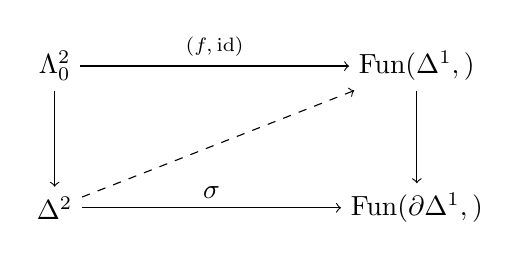
\begin{tikzpicture}
  \node (l) at (0,0) {$\Lambda^2_0$};
  \node (r) at (4.6,0) {$\mathrm{Fun}(\Delta^1, \C)$};
  \node (dl) at (0,-1.8) {$\Delta^2$};
  \node (dr) at (4.6,-1.8) {$\mathrm{Fun}(\partial \Delta^1, \C)$};
  \draw[->] (l) -- node[above] {\scriptsize $(f,\mathrm{id})$} (r);
  \draw[->] (l) -- (dl);
  \draw[->] (r) -- (dr);
  \draw[->] (dl) -- node[above] {$\sigma$} (dr);
  \draw[->, dashed] (dl) -- (r);
\end{tikzpicture}
\end{center}
其中 $f$ 在 $\mathrm{Fun}(\partial \Delta^1, \C)$ 中的像是\trEquivalence{}，
都容有一个解。这蕴含 $f$ 自身容有一个左逆 $g$，其在
$\mathrm{Fun}(\partial \Delta^1, \C)$ 中的像仍是\trEquivalence{}。对 $g$ 施以
同样的推理，我们发现 $g$，从而 $f$，是可逆的。

为了求解该\trLiftingProblem{}，由\trAdjunction{}，我们可以等价地求解下述%
\trLiftingProblem{}：
\begin{center}
\begin{tikzpicture}
  \node (l) at (0,0) {$\Lambda^2_0 \times \Delta^1 \cup \Delta^2 \times \partial \Delta^1$};
  \node (r) at (5.4,0) {$\C$};
  \node (d) at (0,-1.8) {$\Delta^2 \times \Delta^1$};
  \draw[->] (l) -- (r);
  \draw[->] (l) -- (d);
  \draw[->, dashed] (d) -- (r);
\end{tikzpicture}
\end{center}
我们将通过向
$F_0 = \Lambda^2_0 \times \Delta^1 \cup \Delta^2 \times \partial \Delta^1$
粘接一个 $2$-\trSimplex{}与三个 $3$-\trSimplex{}来得到
$\Delta^2 \times \Delta^1$，并一步步把该映射扩张到 $\C$：把
$\Delta^2 \times \Delta^1$ 描写为由图表
\begin{center}
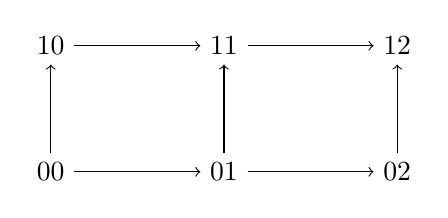
\begin{tikzpicture}
  \node (t1) at (0,0) {$10$};
  \node (t2) at (2.2,0) {$11$};
  \node (t3) at (4.4,0) {$12$};
  \node (b1) at (0,-1.6) {$00$};
  \node (b2) at (2.2,-1.6) {$01$};
  \node (b3) at (4.4,-1.6) {$02$};
  \draw[->] (t1) -- (t2);
  \draw[->] (t2) -- (t3);
  \draw[->] (b1) -- (b2);
  \draw[->] (b2) -- (b3);
  \draw[->] (b1) -- (t1);
  \draw[->] (b2) -- (t2);
  \draw[->] (b3) -- (t3);
\end{tikzpicture}
\end{center}
所描绘的\trCategory{}的\trNerve{}。我们首先粘接由可合成映射
$01 \to 02 \to 12$ 给出的 $2$-\trSimplex{} $\sigma_2$。它与 $F_0$ 的交是内
$2$-\trHorn{}，从而由于 $\C$ 是∞-\trCategory{}，我们可以把给定的映射扩张到
$F_1 = F_0 \cup \sigma_2$。接下来，我们考虑由可合成映射
$00 \to 01 \to 02 \to 12$ 给出的 $3$-\trSimplex{} $\tau_{3,1}$。可以容易地
验证：它与 $F_1$ 的交又是内 $3$-\trHorn{}，故我们可以把给定的映射扩张到
$F_2 = F_1 \cup \tau_{3,1}$。接下来，我们考虑由 $00 \to 01 \to 11 \to 12$
给出的 $\tau_{3,2}$。同样地，我们发现它与 $F_2$ 的交是一个内\trHorn{}，故该
映射可以扩张到 $F_3 = F_2 \cup \tau_{3,2}$。最后，我们考虑由
$00 \to 10 \to 11 \to 12$ 给出的 $\tau_{3,3}$。这一次，它与 $F_3$ 的交由左外\trHorn{}%
$\Lambda^3_0$ 给出，但由假设，特殊边
$\Delta^{[0,1]} \subseteq \Lambda^3_0$ 被送到一个\trEquivalence{}。于是，得益于%
\trJoyal{}提升定理（\cref{thm:special-horn-lifting}），我们可以把给定的映射
扩张到 $F_4 = F_3 \cup \tau_{3,3}$。注意到 $F_4 = \Delta^2 \times \Delta^1$，
本命题即得证。
\end{proof}

\begin{corollary}\label{cor:mapping-infinity-groupoid}
\cref{prop:mapping-infinity-groupoid} 成立。更精确地，给定\trSimplicialSets{}%
的一个在 $0$-\trSimplex{}上为双射的\trMonomorphism{} $L \to K$，那么诱导映射
$\mathrm{Fun}(K, \C) \to \mathrm{Fun}(L, \C)$ 在任意一点
$\Delta^0 \to \mathrm{Fun}(L, \C)$ 之上的\trFibre{}是一个∞-\trGroupoid{}。特别地，
对于一个∞-\trCategory{} $\C$，∞-\trCategory{} $\mathrm{map}_{\C}(x, y)$ 是一个
∞-\trGroupoid{}。
\end{corollary}

\begin{proof}
由\cref{thm:bijective-on-vertices}，\trFunctor{}%
$\mathrm{Fun}(K, \C) \to \mathrm{Fun}(L, \C)$ 是一个\trConservative{}\trInnerFibration{}，
从而沿 $\Delta^0 \to \mathrm{Fun}(L, \C)$ 取\trPullback{}得到的也是一个\trConservative%
\trInnerFibration{}（由\cref{cor:pullback-conservative-inner-fibration}）。%
但 $X \to \ast$ 是\trConservative{}\trInnerFibration{}，当且仅当 $X$ 是∞-\trGroupoid{}。
\end{proof}

注意，\cref{cor:mapping-infinity-groupoid} 的「特别地」部分是
\cref{prop:fun-delta1-boundary-conservative} 的直接应用。

我们以\trIsofibration{}的若干稳定性性质来结束本节。

\begin{proposition}\label{prop:isofibration-induced-functor}
设 $p\colon \C \to \D$ 是一个\trInnerFibration{}，并设 $i\colon K \to L$ 是%
\trSimplicialSets{}的一个\trMonomorphism{}。假设
\begin{enumerate}[label=(\arabic*)]
  \item $p$ 是\trIsofibration{}，或者
  \item $i$ 在 $0$-\trSimplex{}上诱导一个双射。
\end{enumerate}
那么诱导\trFunctor{}%
\[
\C^L \longrightarrow \C^K \times_{\D^K} \D^L
\]
是\trIsofibration{}。
\end{proposition}

\begin{proof}
由\cref{thm:angle-fi-fibration}，我们知道该映射是一个\trInnerFibration{}。于是
只需证明：任何\trLiftingProblem{}%
\begin{center}
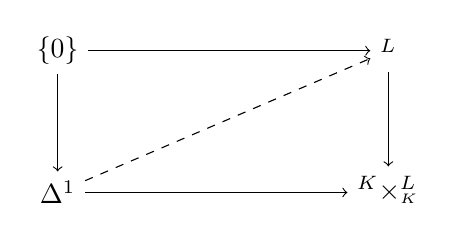
\begin{tikzpicture}
  \node (v) at (0,0) {$\{0\}$};
  \node (c) at (4.2,0) {$\C^L$};
  \node (d1) at (0,-1.8) {$\Delta^1$};
  \node (fp) at (4.2,-1.8) {$\C^K \times_{\D^K} \D^L$};
  \draw[->] (v) -- (c);
  \draw[->] (v) -- (d1);
  \draw[->] (c) -- (fp);
  \draw[->] (d1) -- (fp);
  \draw[->, dashed] (d1) -- (c);
\end{tikzpicture}
\end{center}
其中下面的水平映射是\trEquivalence{}，都拥有一个解，且该解又是一个%
\trEquivalence{}。由\cref{thm:bijective-on-vertices}，如果对 $L$ 的每个%
\trObject{}，$\C$ 中诱导的\trMorphism{}都是\trEquivalence{}，情形便是如此。
特别地，我们看到：如果 $K \to L$ 在 $0$-\trSimplex{}上是双射，那么上述%
\trLiftingProblem{}中右边的竖直映射是\trConservative，故
一个\trEquivalence{}的任意提升自动是\trEquivalence{}。由\trAdjunction{}，这个%
\trLiftingProblem{}因而等价于\trLiftingProblem{}%
\begin{center}
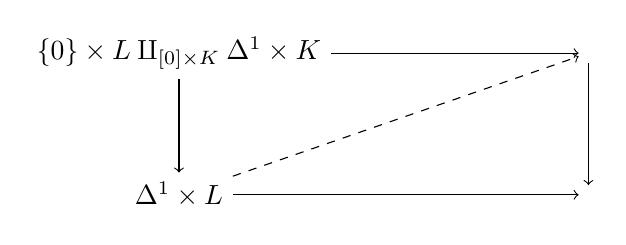
\begin{tikzpicture}
  \node (l) at (0,0)
    {$\{0\} \times L \amalg_{[0] \times K} \Delta^1 \times K$};
  \node (r) at (5.2,0) {$\C$};
  \node (d) at (0,-1.8) {$\Delta^1 \times L$};
  \node (dr) at (5.2,-1.8) {$\D$};
  \draw[->] (l) -- (r);
  \draw[->] (l) -- (d);
  \draw[->] (r) -- (dr);
  \draw[->] (d) -- (dr);
  \draw[->, dashed] (d) -- (r);
\end{tikzpicture}
\end{center}
其中虚映射与映射 $\Delta^1 \times \Delta^0 \to \Delta^1 \times L$ 的复合是%
\trEquivalence{}，后者由 $L$ 的一个任意\trObject{}给出。我们断言：使得结论
成立的那些\trMorphism{} $K \to L$ 构成一个\trSaturatedClass{}。（我们把该断言的验证留作
\cref{ex:isofibration-saturated}。）于是，只需在情形 (1) 中对边界包含
$\partial \Delta^n \to \Delta^n$、而在情形 (2) 中对 $n \ge 1$ 的边界包含，
证明该命题的断言。如果 $n = 0$，那么我们有\trLiftingProblem{}%
\begin{center}
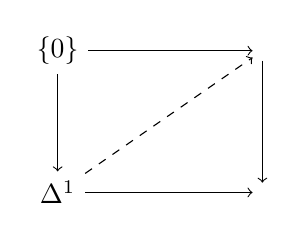
\begin{tikzpicture}
  \node (v) at (0,0) {$\{0\}$};
  \node (c) at (2.6,0) {$\C$};
  \node (d1) at (0,-1.8) {$\Delta^1$};
  \node (d) at (2.6,-1.8) {$\D$};
  \draw[->] (v) -- (c);
  \draw[->] (v) -- (d1);
  \draw[->] (c) -- (d);
  \draw[->] (d1) -- (d);
  \draw[->, dashed] (d1) -- (c);
\end{tikzpicture}
\end{center}
其中下面的水平映射是\trEquivalence{}。代表 $\C$ 中一个\trEquivalence{}的虚箭头
是存在的，因为由假设 $\C \to \D$ 是\trIsofibration{}。对剩下的情形 $n \ge 1$，我们
需要考虑形如下式的图表
\begin{center}
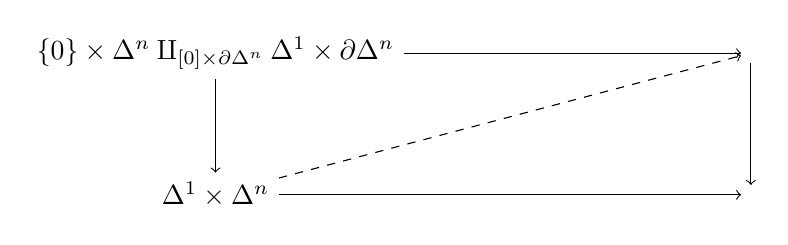
\begin{tikzpicture}
  \node (l) at (0,0)
    {$\{0\} \times \Delta^n \amalg_{[0] \times \partial \Delta^n} \Delta^1 \times \partial \Delta^n$};
  \node (r) at (6.8,0) {$\C$};
  \node (d) at (0,-1.8) {$\Delta^1 \times \Delta^n$};
  \node (dr) at (6.8,-1.8) {$\D$};
  \draw[->] (l) -- (r);
  \draw[->] (l) -- (d);
  \draw[->] (r) -- (dr);
  \draw[->] (d) -- (dr);
  \draw[->, dashed] (d) -- (r);
\end{tikzpicture}
\end{center}
由于我们将不会用到 $p$ 是\trIsofibration{}这一事实，下述论证便处理了 (1) 与 (2) 的
所有剩余情形。人们在 $\Delta^1 \times \Delta^n$ 上构造一个合适的滤过——从
$\{0\} \times \Delta^n \cup \Delta^1 \times \partial \Delta^n$ 出发，逐个添加
缺失的\trSimplex{}（一个具体的这类滤过见例如 \cite[Lemma 62.2]{Rez20}）。于是人们将
发现：相关的\trSimplex{}或者沿内\trHornInclusion{}粘接，或者沿特殊外\trHorn{}粘接（其中从
$0$ 到 $1$ 或从 $n-1$ 到 $n$ 的边被标上一个\trEquivalence{}）。使用\trJoyal{}提升，
本命题即得。
\end{proof}

\begin{corollary}\label{cor:llp-join-inclusion}
设 $K \to L$ 是\trSimplicialSets{}的一个在 $0$-\trSimplex{}上诱导双射的%
\trMonomorphism{}。那么映射
\[
\{0\} \times L \amalg_{[0] \times K} J \times K \longrightarrow J \times L
\]
对∞-\trCategories{}之间的\trInnerFibration{}具有\trLeftLiftingProperty{}。
\end{corollary}

\begin{proof}
让我们考虑一个\trInnerFibration{} $p\colon \C \to \D$ 与\trLiftingProblem{}%
\begin{center}
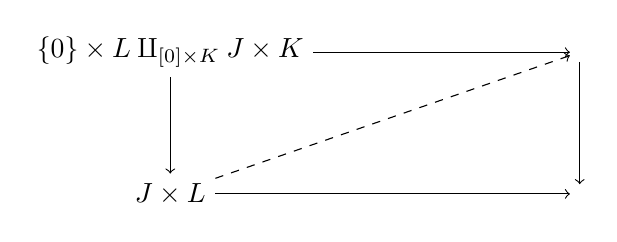
\begin{tikzpicture}
  \node (l) at (0,0)
    {$\{0\} \times L \amalg_{[0] \times K} J \times K$};
  \node (r) at (5.2,0) {$\C$};
  \node (d) at (0,-1.8) {$J \times L$};
  \node (dr) at (5.2,-1.8) {$\D$};
  \draw[->] (l) -- (r);
  \draw[->] (l) -- (d);
  \draw[->] (r) -- (dr);
  \draw[->] (d) -- (dr);
  \draw[->, dashed] (d) -- (r);
\end{tikzpicture}
\end{center}
由\trAdjunction{}，这个\trLiftingProblem{}等价于\trLiftingProblem{}%
\begin{center}
\begin{tikzpicture}
  \node (v) at (0,0) {$\{0\}$};
  \node (c) at (4.2,0) {$\C^L$};
  \node (j) at (0,-1.8) {$J$};
  \node (fp) at (4.2,-1.8) {$\C^K \times_{\D^K} \D^L$};
  \draw[->] (v) -- (c);
  \draw[->] (v) -- (j);
  \draw[->] (c) -- (fp);
  \draw[->] (j) -- (fp);
  \draw[->, dashed] (j) -- (c);
\end{tikzpicture}
\end{center}
而由\cref{prop:isofibration-induced-functor}，右边的竖直映射是\trIsofibration{}。
于是，该\trLiftingProblem{}可以由\cref{prop:isofibration-rlp-j} 求解。
\end{proof}

\begin{corollary}\label{cor:equivalences-in-functor-pullback}
设 $f\colon \C \to \D$ 是∞-\trCategories{}之间的一个\trFunctor{}，而
$K \to L$ 是\trSimplicialSets{}的一个\trMonomorphism{}。那么
\[
(\C^K \times_{\D^K} \D^L)^{\simeq} = (\C^{\simeq})^K \times_{(\D^K)^{\simeq}} (\D^L)^{\simeq}.
\]
\end{corollary}

\begin{proof}
两个\trSimplicialSets{}都是\trPullback{} $\C^K \times_{\D^K} \D^L$ 的子集，
因此我们容易得到包含「$\subseteq$」。为了证明反向包含，只需证明右边事实上是
一个∞-\trGroupoid{}，因为在这一情形中，它当然包含
$\C^K \times_{\D^K} \D^L$ 之中最小的∞-\trGroupoid{}，而后者正是左边。把%
\cref{prop:isofibration-induced-functor} 应用于\trIsofibration{} $\D \to \Delta^0$，
我们发现 $\D^L \to \D^K$ 也是\trIsofibration{}。于是，由
\cref{prop:isofibration-maximal-groupoid-kan}，映射
$(\D^L)^{\simeq} \to (\D^K)^{\simeq}$ 是\trKanComplex{}之间的%
\trKanFibration{}，从而沿来自\trKanComplex{}的映射取任意\trPullback{}仍得到%
\trKanComplex{}。
\end{proof}

\begin{proposition}\label{prop:joyal-equivalence-precomposition}
设 $f\colon \C \to \D$ 是∞-\trCategories{}之间的一个\trFunctor{}。那么 $f$
是一个\trJoyalEquivalence{}，当且仅当对每个∞-\trCategory{} $\E$，
诱导映射
\[
f^*\colon \mathrm{Fun}(\D, \E) \to \mathrm{Fun}(\C, \E)
\]
是一个\trJoyalEquivalence{}。
\end{proposition}

\begin{proof}
为了证明「仅当」部分，选取一个逆 $\D \to \C$ 以及见证 $g$ 逆于 $f$ 的%
\trNaturalTransformation{} $(\eta_0, \eta_1)$。那么四元组
$(f^*, g^*, \eta_0^*, \eta_1^*)$ 便确定 $\mathrm{Fun}(\C, \E)$ 与
$\mathrm{Fun}(\D, \E)$ 之间的一个\trEquivalence{}。

我们现在证明：如果对所有∞-\trCategories{} $\E$，\trFunctor{} $f^*$
都是\trJoyalEquivalence{}，那么 $f$ 事实上是\trJoyalEquivalence{}。由
\cref{ex:joyal-equivalence-core}，我们得到一个双射
\[
f^*\colon \pi_0(\mathrm{Fun}(\D, \E)^{\simeq})
\stackrel{\cong}{\longrightarrow} \pi_0(\mathrm{Fun}(\C, \E)^{\simeq})
\]
现在考虑 $\E = \C$ 的情形：该双射证明了这样一个\trFunctor{}%
$g\colon \D \to \C$ 的存在性，使得 $f^*(g) = gf$ 等价于 $\mathrm{id}_{\C}$。
取 $\E = \D$，我们看到
\[
f^*(fg) = fgf \simeq f,
\]
从而正如所需，有 $fg \simeq \mathrm{id}_{\D}$。
\end{proof}

\begin{definition}\label{def:joyal-equivalence-simplicial-sets}
\trSimplicialSets{}之间的一个映射 $f\colon X \to Y$ 称为\emph{\trJoyalEquivalence{}}（Joyal equivalence，或称\trCategoricalEquivalence{}），如果对所有∞-\trCategories{} $\C$，诱导映射
\[
\mathrm{Fun}(Y, \C) \longrightarrow \mathrm{Fun}(X, \C)
\]
是∞-\trCategories{}之间的\trJoyalEquivalence{}。
\end{definition}

\begin{observation}\label{obs:joyal-equivalence-unchanged}
由\cref{prop:joyal-equivalence-precomposition}，当 $X$ 与 $Y$ 已经是
∞-\trCategories{}时，该定义不改变原有的定义。
\end{observation}

\begin{observation}\label{obs:joyal-equivalence-kan-homotopy}
\trKanComplex{}之间的\trJoyalEquivalence{}恰好是\trHomotopy{}等价。
\end{observation}

\begin{proposition}\label{prop:trivial-kan-fibration-joyal-equivalence}
一个平凡\trKanFibration{} $f\colon X \to Y$ 是\trJoyalEquivalence{}。
\end{proposition}

\begin{proof}
考虑\trSimplicialSets{}的下述\trPullback{}方形：
\begin{center}
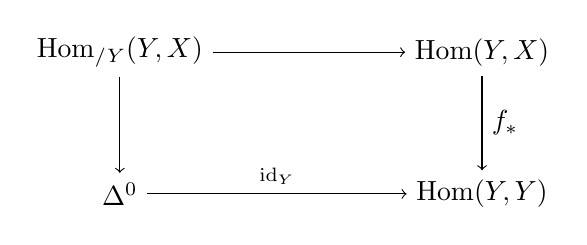
\begin{tikzpicture}
  \node (a) at (0,0) {$\mathrm{Hom}_{/Y}(Y, X)$};
  \node (b) at (4.6,0) {$\mathrm{Hom}(Y, X)$};
  \node (c) at (0,-1.8) {$\Delta^0$};
  \node (d) at (4.6,-1.8) {$\mathrm{Hom}(Y, Y)$};
  \draw[->] (a) -- (b);
  \draw[->] (a) -- (c);
  \draw[->] (b) -- node[right] {$f_*$} (d);
  \draw[->] (c) -- node[above] {\scriptsize $\mathrm{id}_Y$} (d);
\end{tikzpicture}
\qquad
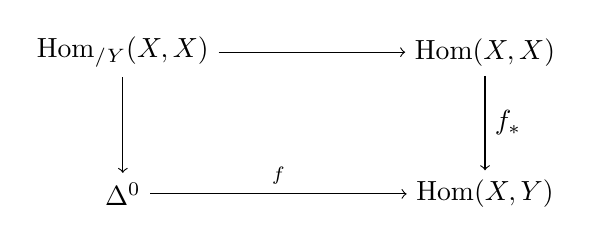
\begin{tikzpicture}
  \node (a) at (0,0) {$\mathrm{Hom}_{/Y}(X, X)$};
  \node (b) at (4.6,0) {$\mathrm{Hom}(X, X)$};
  \node (c) at (0,-1.8) {$\Delta^0$};
  \node (d) at (4.6,-1.8) {$\mathrm{Hom}(X, Y)$};
  \draw[->] (a) -- (b);
  \draw[->] (a) -- (c);
  \draw[->] (b) -- node[right] {$f_*$} (d);
  \draw[->] (c) -- node[above] {\scriptsize $f$} (d);
\end{tikzpicture}
\end{center}
每个方形中右边的竖直映射都是\trTrivialFibration{}，故它们的\trPullback{}也是如此。
但 $\Delta^0$ 之上的\trTrivialFibration{}以一个可缩\trKanComplex{}作为源。选取一个
$0$-\trSimplex{} $s \in \mathrm{Hom}_{/Y}(Y, X)$，使得
$f_*(s) = fs = \mathrm{id}_Y$。（为此，回忆 $f_*$ 像每个\trTrivialFibration{}一样容有一个%
\trSectionMap{}，而且任何满足 $fs = \mathrm{id}_Y$ 的 $0$-\trSimplex{}%
$s \in \mathrm{Hom}(Y, X)$ 都落在 $\mathrm{Hom}_{/Y}(Y, X)$ 之中。）那么
$sf$ 便确定 $\mathrm{Hom}_{/Y}(X, X)$ 中的一个 $0$-\trSimplex{}，于是必定存在
一条把它连到恒等的 $1$-\trSimplex{}（仍因为这些\trSectionMap{}空间是可缩的）。显式地，
我们可以找到一个映射
\[
\Delta^1 \longrightarrow \mathrm{Hom}_{/Y}(X, X)
\]
其在 $0$ 处的限制为 $sf$，而在 $1$ 处的限制为 $\mathrm{id}_X$。对一个任意的
∞-\trCategory{}，我们可以把这个映射与典范映射
\[
\mathrm{Hom}_{/Y}(X, X) \longrightarrow \mathrm{Hom}(X, X)
\longrightarrow \mathrm{Hom}(\C^X, \C^X)
\]
复合，并看到所得到的映射
\[
\Delta^1 \longrightarrow \mathrm{Hom}_{/Y}(X, X)
\longrightarrow \mathrm{Hom}(\C^X, \C^X)^{\simeq}
\]
确定 $(sf)^*$ 与 $\mathrm{id}_{\C^X}$ 之间的一个\trNaturalEquivalence{}。由于
$(fs)^* = \mathrm{id}_{\C^Y}$，我们已经证明：对任意∞-\trCategory{} $\C$，
$f^*$ 与 $s^*$ 确定 $\C^X$ 与 $\C^Y$ 的互逆\trEquivalence{}，从而 $f^*$ 是一个%
\trJoyalEquivalence{}。\footnote{译注：原书此处印作「对任意∞-范畴 $Y$」，但
$Y$ 是底\trSimplicialSet{}，所述的任意∞-范畴应为 $\C$（即 $\C^X$、$\C^Y$ 中的上标底座），
兹径改。——译者注}因此，$f$ 自身是\trJoyalEquivalence{}。
\end{proof}

\begin{corollary}\label{cor:inner-anodyne-joyal-equivalence}
内\trAnodyneMap{}是\trJoyalEquivalence{}。
\end{corollary}

\begin{proof}
设 $i\colon A \to B$ 是一个内\trAnodyneMap{}，而 $\C$ 是一个∞-\trCategory{}。
我们需要证明 $\C^B \to \C^A$ 是\trJoyalEquivalence{}。由
\cref{thm:angle-fi-fibration} 第 (2) 部分，该映射是\trTrivialFibration{}，于是断言由
\cref{prop:trivial-kan-fibration-joyal-equivalence} 得证。
\end{proof}

\begin{corollary}\label{cor:simplicial-set-joyal-equivalent}
每个\trSimplicialSet{}都与某个∞-\trCategory{}\trJoyalEquivalence{}。
\end{corollary}

\begin{proof}
由\trSmallObjectArgument{}（\cref{prop:small-object-argument}），对任意%
\trSimplicialSet{} $X$，人们可以把映射 $X \to \ast$ 分解为一个内%
\trAnodyneMap{}接上一个\trInnerFibration{}。这给出一个映射 $X \to \C$，其中
$\C$ 是∞-\trCategory{}，而 $X \to \C$ 是\trInnerAnodyne{}的。由
\cref{cor:inner-anodyne-joyal-equivalence}，该映射是\trJoyalEquivalence{}。
\end{proof}

\begin{lemma}\label{lem:kan-fibration-surjection-pi0}
\trKanComplex{}之间的一个在 $\pi_0$ 上诱导满射的\trKanFibration{}%
$p\colon X \to Y$ 事实上在 $0$-\trSimplex{}上是满的。同样，\trKanComplex{}之间
的一个在 $\pi_0$ 上诱导单射而在 $\pi_1$ 上诱导满射的\trKanFibration{}具有如下
性质：任何\trLiftingProblem{}%
\begin{center}
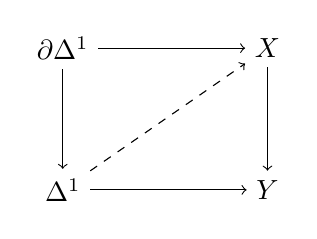
\begin{tikzpicture}
  \node (l) at (0,0) {$\partial \Delta^1$};
  \node (r) at (2.6,0) {$X$};
  \node (d) at (0,-1.8) {$\Delta^1$};
  \node (dr) at (2.6,-1.8) {$Y$};
  \draw[->] (l) -- (r);
  \draw[->] (l) -- (d);
  \draw[->] (r) -- (dr);
  \draw[->] (d) -- (dr);
  \draw[->, dashed] (d) -- (r);
\end{tikzpicture}
\end{center}
都可求解。
\end{lemma}

\begin{proof}
由于任何\trHomotopy{}等价在单纯道路分支上诱导一个双射，对一个 $0$-\trSimplex{}%
$y\colon \Delta^0 \to Y$，我们得到一个交换图表
\begin{center}
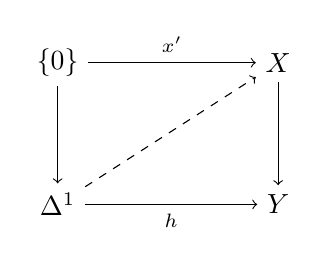
\begin{tikzpicture}
  \node (v) at (0,0) {$\{0\}$};
  \node (x) at (2.8,0) {$X$};
  \node (d1) at (0,-1.8) {$\Delta^1$};
  \node (y) at (2.8,-1.8) {$Y$};
  \draw[->] (v) -- node[above] {\scriptsize $x'$} (x);
  \draw[->] (v) -- (d1);
  \draw[->] (x) -- (y);
  \draw[->] (d1) -- node[below] {\scriptsize $h$} (y);
  \draw[->, dashed] (d1) -- (x);
\end{tikzpicture}
\end{center}
其中 $h|_{\{1\}} = y$。由于 $p$ 是\trKanFibration{}，虚箭头存在。其在 $\{1\}$ 上
的限制提供了 $y$ 在 $X$ 中的一个原像。

至于第二个断言，选取 $X$ 的两个\trObject{} $x, x'$，它们给出交换图表
\begin{center}
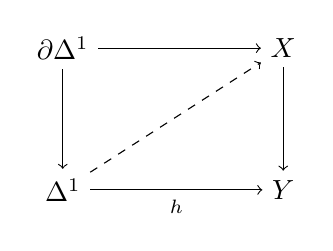
\begin{tikzpicture}
  \node (l) at (0,0) {$\partial \Delta^1$};
  \node (r) at (2.8,0) {$X$};
  \node (d) at (0,-1.8) {$\Delta^1$};
  \node (dr) at (2.8,-1.8) {$Y$};
  \draw[->] (l) -- (r);
  \draw[->] (l) -- (d);
  \draw[->] (r) -- (dr);
  \draw[->] (d) -- node[below] {\scriptsize $h$} (dr);
  \draw[->, dashed] (d) -- (r);
\end{tikzpicture}
\end{center}
中的顶行映射。我们希望证明该图表容有一个虚箭头。$p$ 在 $\pi_1$ 上诱导满射这一
假设蕴含：同一结论不仅对 $x$ 的某一点处的\trLoop{}成立，而且对从 $x$ 到 $x'$ 的
道路的\trHomotopy{}类也成立。（这正是我们使用 $p$ 在道路分支上诱导单射这一事实的
地方：也就是说，这些假设蕴含 $X$ 中存在一条从 $x$ 到 $x'$ 的道路，我们可以用
它把从 $x$ 到 $x'$ 的道路的\trHomotopy{}类之集与 $x$ 处的\trLoop{}的\trHomotopy{}类之集作比较。）
于是人们可以找到一条道路 $\alpha\colon \Delta^1 \to X$，它在施以 $p$ 之后变得
等价于 $h$。这意味着我们可以找到一个\trTwoCell{} $\sigma\colon \Delta^2 \to Y$，使得
$\sigma|_{\Delta^{[0,1]}} = p(\alpha)$，$\sigma|_{\Delta^{[0,2]}} = h$ 且
$\sigma|_{\Delta^{[1,2]}} = \mathrm{id}_{x'}$。由于我们既能提升 $p(\alpha)$
又能提升恒等，我们便得到一个\trLiftingProblem{}%
\begin{center}
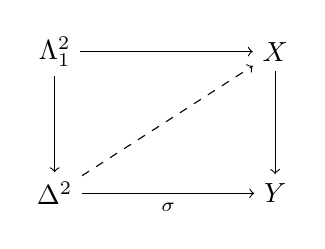
\begin{tikzpicture}
  \node (l) at (0,0) {$\Lambda^2_1$};
  \node (r) at (2.8,0) {$X$};
  \node (d) at (0,-1.8) {$\Delta^2$};
  \node (dr) at (2.8,-1.8) {$Y$};
  \draw[->] (l) -- (r);
  \draw[->] (l) -- (d);
  \draw[->] (r) -- (dr);
  \draw[->] (d) -- node[below] {\scriptsize $\sigma$} (dr);
  \draw[->, dashed] (d) -- (r);
\end{tikzpicture}
\end{center}
它可以求解，因为 $p$ 是\trKanFibration{}。所得到的映射便解决了原来的%
\trLiftingProblem{}。
\end{proof}

\begin{remark}\label{rem:kan-fibration-we-trivial-fibration}
事实上，一个同时是\trWeakEquivalence{}的\trKanFibration{}是\trTrivialFibration{}。这是
单纯\trHomotopyTheory{}中的一个经典事实，我们可以由前一个引理连同下述观察把它推导出来。
\end{remark}

\begin{lemma}\label{lem:trivial-fibration-joyal-isofibration}
∞-\trCategories{}之间的一个\trFunctor{} $p\colon \C \to \D$ 是\trTrivialFibration{}，
当且仅当它既是\trJoyalEquivalence{}又是\trIsofibration{}。
\end{lemma}

\begin{proof}
由\cref{prop:trivial-kan-fibration-joyal-equivalence}，\trTrivialFibration{}是%
\trJoyalEquivalence{}，而它们是\trIsofibration{}，因为\trTrivialFibration{}是一个%
\trLeftFibration{}，后者又由\cref{prop:left-right-fibrations-conservative-isofibrations}
是\trConservative{}\trIsofibration{}。

为了看出证明的逆方向，我们需要证明：对任何\trMonomorphism{} $K \to L$，
\trLiftingProblem{}%
\begin{center}
\begin{tikzpicture}
  \node (k) at (0,0) {$K$};
  \node (c) at (2.6,0) {$\C$};
  \node (l) at (0,-1.8) {$L$};
  \node (d) at (2.6,-1.8) {$\D$};
  \draw[->] (k) -- (c);
  \draw[->] (k) -- (l);
  \draw[->] (c) -- node[right] {$p$} (d);
  \draw[->] (l) -- (d);
  \draw[->, dashed] (l) -- (c);
\end{tikzpicture}
\end{center}
都有解。这等价于\trLiftingProblem{}%
\begin{center}
\begin{tikzpicture}
  \node (e) at (0,0) {$\varnothing$};
  \node (cl) at (4.2,0) {$\C^L$};
  \node (d0) at (0,-1.8) {$\Delta^0$};
  \node (fp) at (4.2,-1.8) {$\C^K \times_{\D^K} \D^L$};
  \draw[->] (e) -- (cl);
  \draw[->] (e) -- (d0);
  \draw[->] (cl) -- node[right] {$\bar{p}$} (fp);
  \draw[->] (d0) -- (fp);
  \draw[->, dashed] (d0) -- (cl);
\end{tikzpicture}
\end{center}
而这归结为证明右边的映射在 $0$-\trSimplex{}上的满性。为证明这一断言，我们可以
过渡到底\trGroupoid{}核，因为这个过渡不改变 $0$-\trSimplex{}。

由\cref{prop:isofibration-induced-functor}，$\bar{p}$ 是\trIsofibration{}，因为 $p$
是\trIsofibration{}。特别地，诱导映射
\[
(\C^L)^{\simeq} \stackrel{\bar{p}}{\longrightarrow}
(\C^K \times_{\D^K} \D^L)^{\simeq}
\]
是一个\trKanFibration{}。\footnote{译注：原书此式右端印作
$\C^K \times_{\D^K} \C^L$，据\cref{prop:isofibration-induced-functor} 与同页
下一式，末项应为 $\D^L$，兹径改。——译者注}此外，由
\cref{cor:equivalences-in-functor-pullback}，后一个映射（沿典范映射）等于\trGroupoid{}核
的\trPullback{}，因此我们发现映射
\[
(\C^L)^{\simeq} \longrightarrow
(\C^K)^{\simeq} \times_{(\D^K)^{\simeq}} (\D^L)^{\simeq}
\]
是一个\trKanFibration{}。我们希望证明该映射在 $0$-\trSimplex{}上是满的。由
\cref{lem:kan-fibration-surjection-pi0}，只需证明它在 $\pi_0$ 上诱导一个满射。
为此，我们观察到：由于 $\C \to \D$ 是\trJoyalEquivalence{}，映射
\[
\C^K \to \D^K \quad\text{与}\quad \C^L \to \D^L
\]
由\cref{ex:joyal-equivalence-fun}也是\trJoyalEquivalence{}。由于它们是\trIsofibration{}，过渡到\trGroupoid{}核便给出%
\trKanFibration{}，而这些\trKanFibration{}此外还是\trJoyalEquivalence{}。

接下来，我们考虑图表
\begin{center}
\begin{tikzpicture}
  \node (a) at (0,0) {$(\C^L)^{\simeq}$};
  \node (b) at (5.4,0)
    {$(\C^K)^{\simeq} \times_{(\D^K)^{\simeq}} (\D^L)^{\simeq}$};
  \node (c) at (10.4,0) {$(\D^L)^{\simeq}$};
  \node (d) at (5.4,-1.9) {$(\C^K)^{\simeq}$};
  \node (e) at (10.4,-1.9) {$(\D^K)^{\simeq}$};
  \draw[->] (a) -- (b);
  \draw[->] (b) -- (c);
  \draw[->] (b) -- (d);
  \draw[->] (c) -- (e);
  \draw[->] (d) -- (e);
\end{tikzpicture}
\end{center}
并注意所有映射都是\trKanFibration{}，而且复合与下面的水平映射都是%
\trJoyalEquivalence{}，从而是\trHomotopy{}等价。我们希望证明：顶行第二个映射在 $\pi_0$
上诱导一个双射，从而第一个映射在 $\pi_0$ 上诱导一个满射。为此，我们观察到：
由\cref{lem:kan-fibration-surjection-pi0}，下面的水平映射对
$\partial \Delta^1 \to \Delta^1$ 具有\trRightLiftingProperty{}。作为一个%
\trPullback{}，同样的结论适用于顶行第二个映射，这蕴含该映射在 $\pi_0$ 上是
单的。

使用\cref{lem:kan-fibration-surjection-pi0}，我们发现映射
\[
(\C^L)^{\simeq} \longrightarrow
(\C^K)^{\simeq} \times_{(\D^K)^{\simeq}} (\D^L)^{\simeq}
\]
在 $0$-\trSimplex{}上诱导一个满射。这就证明了本引理。
\end{proof}

\begin{corollary}\label{cor:trivial-kan-homotopy-equivalence}
\trKanComplex{}之间的一个\trKanFibration{} $p\colon X \to Y$ 是平凡\trKanFibration{}，
当且仅当它是一个\trHomotopy{}等价。特别地，在诸\trKanFibration{}之中，平凡\trKanFibration{}%
满足\trThreeForTwoProperty{}（3-for-2 property）。
\end{corollary}

在上述语境中，一个映射之集 $S$ 称为具有\trThreeForTwoProperty{}（3-for-2 property），如果对
任意两个可合成的映射 $g$ 与 $f$，只要三个映射 $f$，$g$ 与 $gf$ 之中的两个属于
$S$，那么第三个也属于 $S$。

\begin{proof}
是\trHomotopy{}等价的\trKanFibration{}是一个\trIsofibration{}，且是一个\trJoyalEquivalence{}。
「特别地」部分由\trHomotopy{}等价的\trThreeForTwoProperty{}得出。
\end{proof}

\begin{remark}\label{rem:isofibration-joyal-trivial-fibration}
\cref{cor:trivial-kan-homotopy-equivalence} 蕴含：给定一个此外还是%
\trJoyalEquivalence{}的\trIsofibration{} $p\colon \C \to \D$，诱导映射
\[
(\C^L)^{\simeq} \stackrel{\bar{p}}{\longrightarrow}
(\C^K \times_{\D^K} \D^L)^{\simeq}
\]
事实上是\trTrivialFibration{}。\footnote{译注：原书此式的末项印作
$\C^L$；与\cref{lem:trivial-fibration-joyal-isofibration} 的证明中的情形相同，
应为 $\D^L$，兹径改。——译者注}这是由于：$\C \to \D$ 是\trJoyalEquivalence{}，
故映射
\[
\C^K \to \D^K \quad\text{与}\quad \C^L \to \D^L
\]
也是\trJoyalEquivalence{}。于是，在复合
\[
(\C^L)^{\simeq} \longrightarrow
(\C^K)^{\simeq} \times_{(\D^K)^{\simeq}} (\D^L)^{\simeq}
\longrightarrow
(\D^L)^{\simeq}
\]
中，复合与后一个映射都是\trTrivialFibration{}：就复合而言，它是一个作为\trHomotopy{}等价的%
\trKanFibration{}，从而是\trTrivialFibration{}；就后一个映射而言，它是映射
$(\C^K)^{\simeq} \to (\D^K)^{\simeq}$ 的一个\trPullback{}，而由同样的推理，
后者是平凡\trKanFibration{}。由\trTrivialFibration{}（在诸\trKanFibration{}之中）的\trThreeForTwoProperty{}，
便得出映射
\[
(\C^L)^{\simeq} \longrightarrow
(\C^K)^{\simeq} \times_{(\D^K)^{\simeq}} (\D^L)^{\simeq}
\]
也是\trTrivialFibration{}。
\end{remark}
